\documentclass[
 size=12pt,
 paper=smartboard, %a4paper, smartboard, screen
 mode=present, %present, handout, print
 display=slides, % slidesnotes, notes, slides
% nohandoutpagebreaks,
% pauseslide,
style=tuliplab,
% nopagebreaks,clock
% hlentries=true,
% hlsections = true,
pauseslide,
fleqn,leqno]{powerdot}

\hypersetup{pdfpagemode=FullScreen}
% \usepackage[toc,highlight,blackslide,slidesonly,sounds,HA]{HA-prosper}

\usepackage{amssymb}
\usepackage{amsmath} 
\usepackage{rotating}
\usepackage{graphicx}
\usepackage{boxedminipage}
\usepackage{media9}
\usepackage{rotate}
\usepackage{calc}
\usepackage[absolute]{textpos}
\usepackage{psfrag,overpic}
\usepackage{fouriernc}
\usepackage{pstricks,pst-node,pst-text,pst-3d,pst-grad}
\usepackage{moreverb,epsfig,color,subfigure}
\usepackage{color}
\usepackage{pstricks}
\usepackage{pstricks-add}
\usepackage{pst-text}
\usepackage{pst-node, pst-tree}
\usepackage{booktabs}
\usepackage{etex}
\usepackage{breqn}
\usepackage{multirow}
\usepackage{gitinfo2}
\usepackage{bmpsize}
\usepackage{listings}
\lstset{frameround=fttt, 
frame=trBL, 
stringstyle=\ttfamily,
backgroundcolor=\color{yellow!20},
basicstyle=\footnotesize\ttfamily}
\lstnewenvironment{code}{
\lstset{frame=single,escapeinside=`',
backgroundcolor=\color{yellow!20},
basicstyle=\footnotesize\ttfamily}
}{}

\usepackage{fouriernc}
\usepackage{hyperref}

%%%%%%%%%%%%%%%%%%%%%%%%%%%%%%%%%%%%%%%%%%%%%%%%%%%%%%%%%%%%%%%%%%%%%%%%
% title
% TODO: Customize to your Own Title, Name, Address
%
\title{FLIP(01) Mid-Term Presentation}
\author{
Jiahui Zhou
\\
Xian Shiyou University 
% \href{mailto:gangli@acm.org}{gangli@acm.org}
% \and % more authors
}
\date{\gitCommitterDate}


% Customize the setting of slides
\pdsetup{
% theslide=\arabic{slide}~/~\pageref*{lastslide},
% theslide=\arabic{slide},
rf=\href{http://www.tulip.org.au}{
Last Changed by: \textsc{\gitCommitterName}\ \gitVtagn-\gitAbbrevHash\ (\gitAuthorDate)
},
cf=\hyperlink{blankslide}{FLIP(01) Mid-Term Presentation},
trans=Fade,
list={labelsep=1em,leftmargin=*,itemsep=0pt,topsep=5pt,parsep=0pt},
% counters={theorem,lemma},
% randomdots,dmaxdots=80
}


\begin{document}

\maketitle 

\begin{slide}[toc=,bm=]{Content}
\tableofcontents[content=sections,type=1]
\end{slide}

\section{Overview}
\begin{slide}{Problem Defination}
    \begin{itemize}
        \item \textbf{Problem:}\ Google QUEST Q\&A Labeling
        \begin{itemize}
            \item Text Processing
            \item Question-answer pairs dataset
            \item Multi-task Regression
        \end{itemize}
    \end{itemize} 
    \centering{
        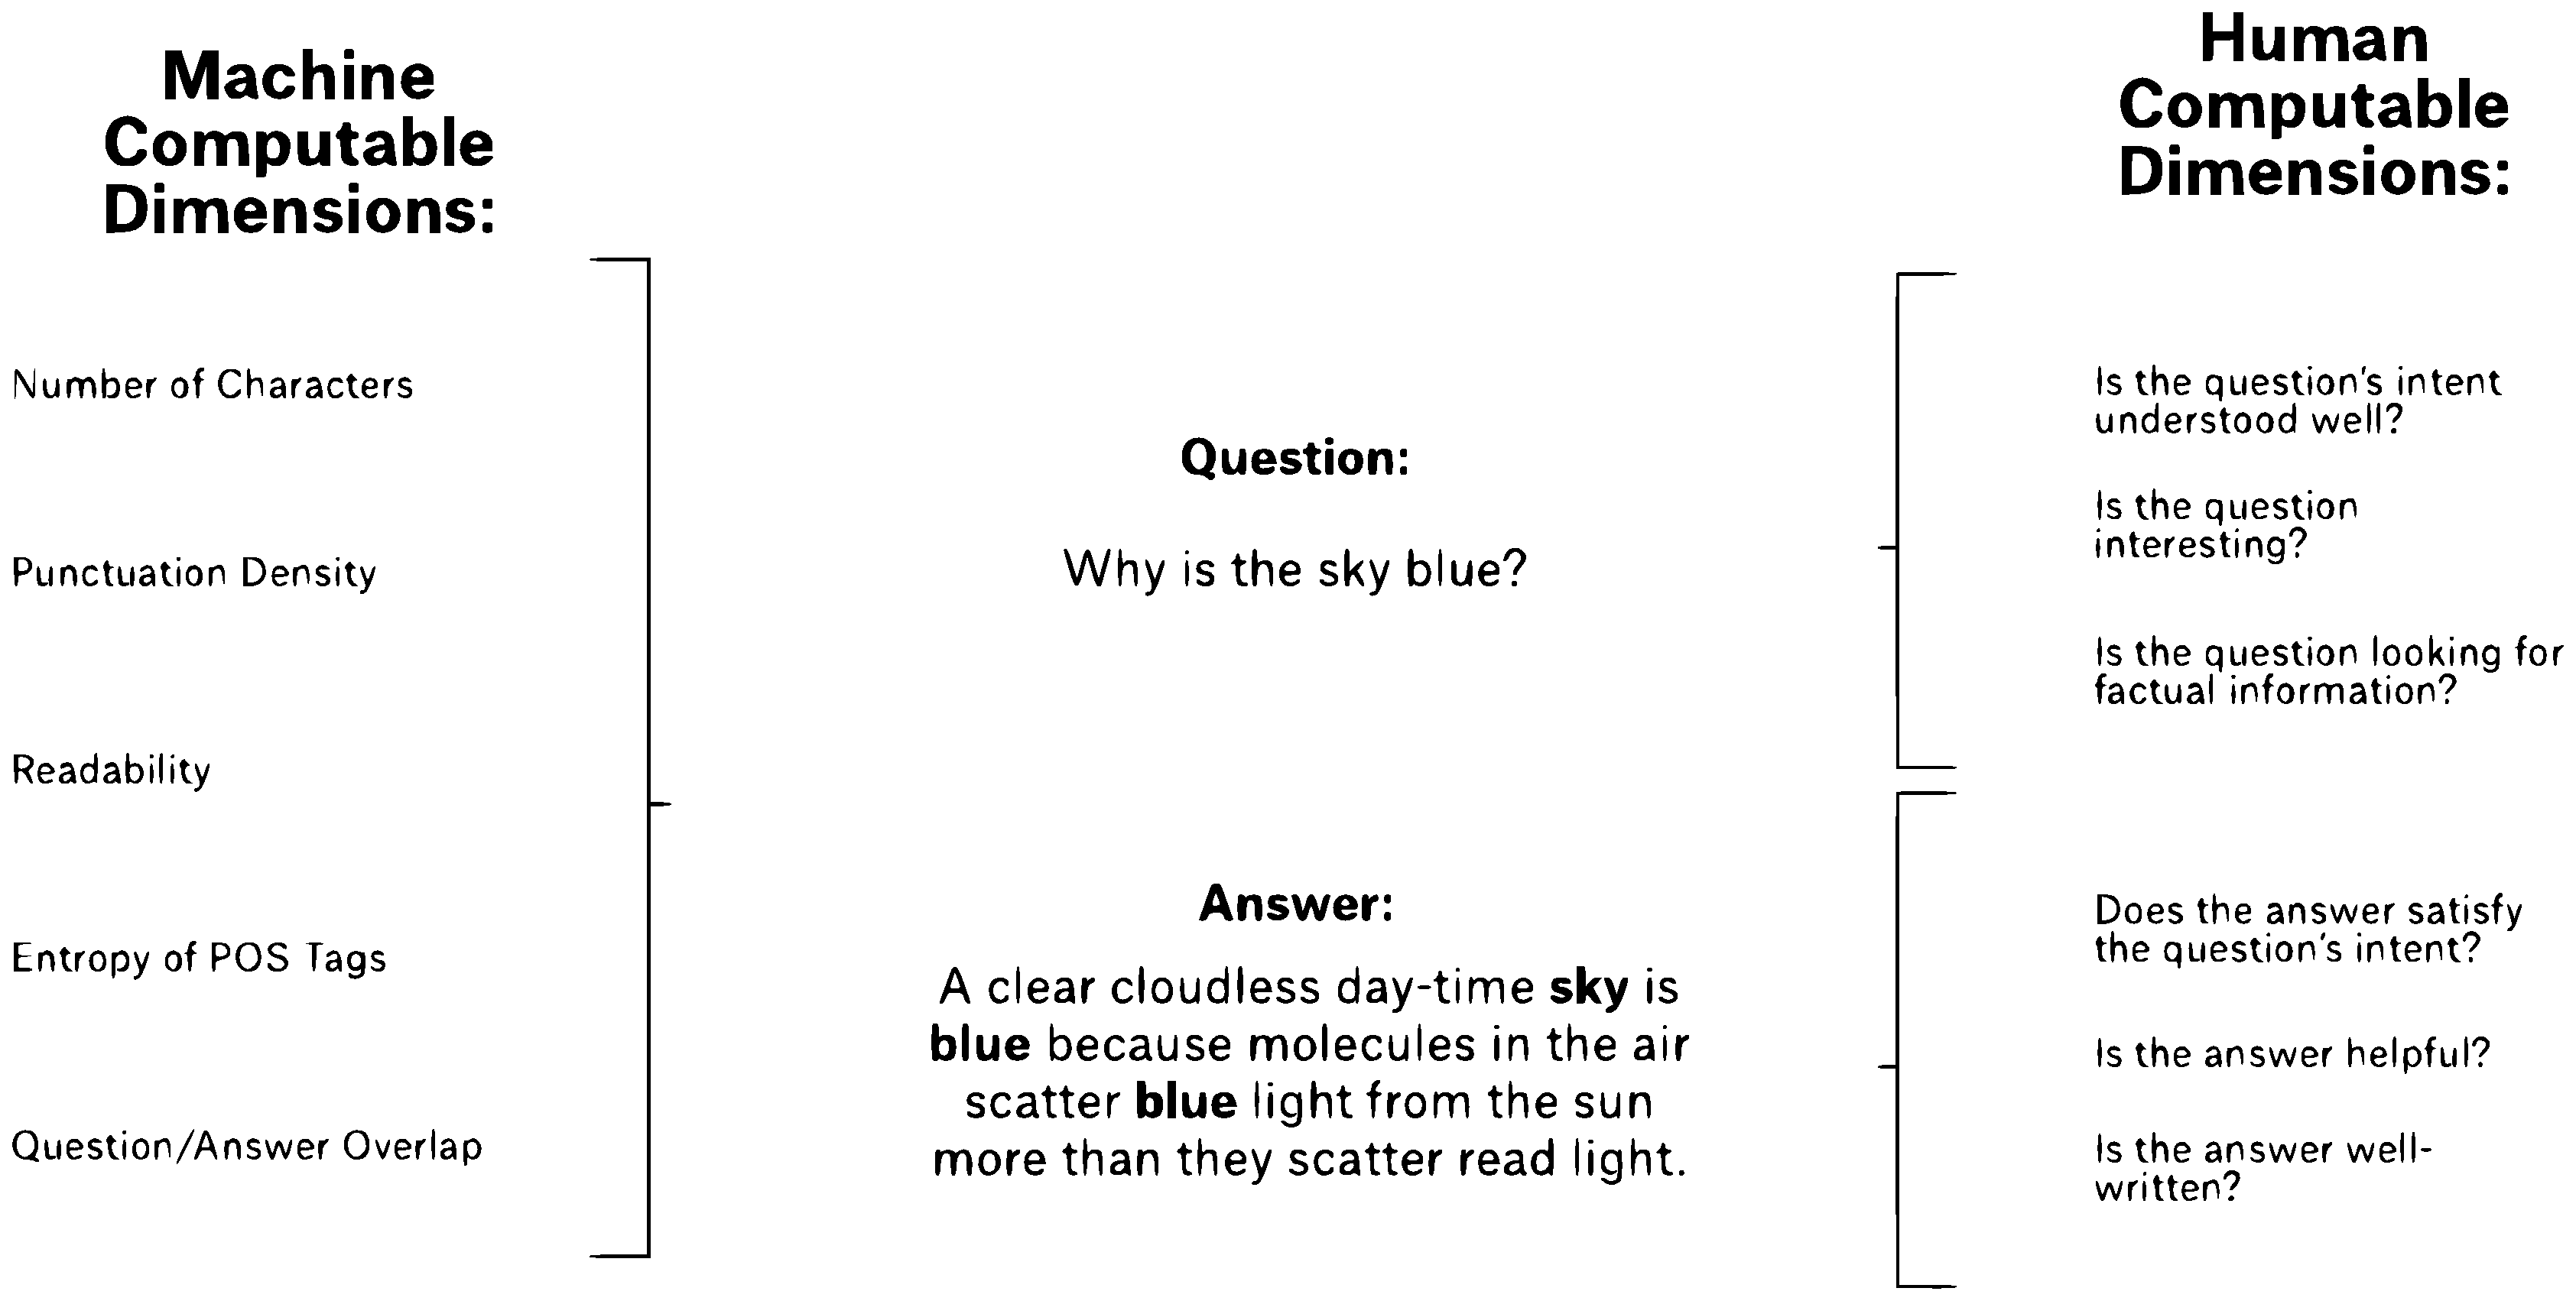
\includegraphics[height=0.5\slideheight]{figures/title.eps}  
    } 
\end{slide}
\begin{slide}{Dataset}
    \begin{itemize}
        \item 6049 records in training set
        \item 476 records in test set
        \item Features:
        \begin{itemize}
            \item Question title\&body
            \item Answer
            \item Host
            \item Category
            \item Question user
            \item Answer user
            \item Url
        \end{itemize}
        \item Targets:
        \begin{itemize}
            \item Continuous values in the range [0,1]
            \item 21 question related target
            \item 9 answer related target
        \end{itemize}
    \end{itemize}
\end{slide}
\begin{slide}{Possible Solution}
    \begin{itemize}
        \item One model for each target
        \begin{itemize}
            \item Bayesian linear Regression
        \end{itemize}
        \item Multi-task learning
        \begin{itemize}
            \item Neural network
        \end{itemize}
    \end{itemize}
\end{slide}
\section{EDA \& Feature Engineering}
\begin{slide}{Host and Category}
    \centering{
        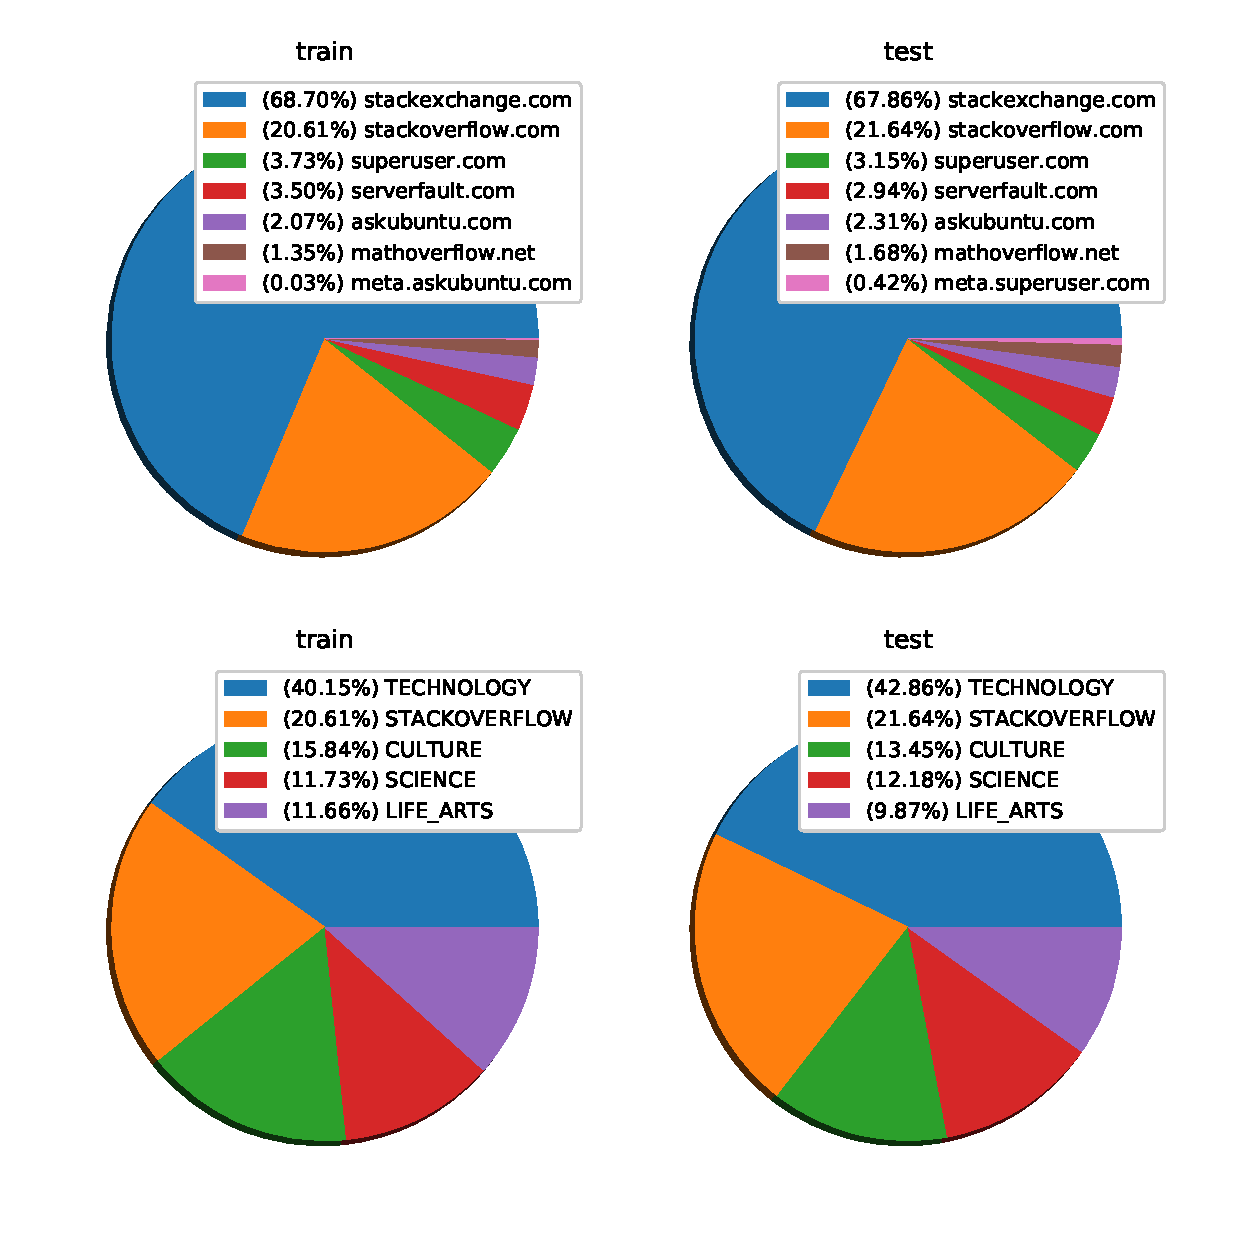
\includegraphics[height=0.6\slideheight]{figures/hosts_categories.eps}
    }
\end{slide}
\begin{slide}{Targets Detail}
    \twocolumn[lineheight=0.7\slideheight,topsep=0.1cm]{
        \textbf{21 question related targets:}
        \begin{itemize}
            \item question_asker_intent_understanding
            \item question_body_critical
            \item question_conversational
            \item question_expect_short_answer
            \item question_fact_seeking
            \item question_has_commonly_accepted_answer
            \item question_interestingness_others
            \item question_interestingness_self
            \item question_multi_intent
            \item question_not_really_a_question
            \item question_opinion_seeking 
            \item question_type_choice
            \item question_type_compare 
            \item question_type_consequence
            \item question_type_definition 
            \item question_type_entity
            \item question_type_instructions 
            \item question_type_procedure
            \item question_type_reason_explanation
            \item question_type_spelling
            \item question_well_written
        \end{itemize}    
    }
    {
        \textbf{9 answer related targets:}
        \begin{itemize}
            \item answer_helpful
            \item answer_level_of_information
            \item answer_plausible
            \item answer_relevance
            \item answer_satisfaction
            \item answer_type_instructions
            \item answer_type_procedure 
            \item answer_type_reason_explanation
            \item answer_well_written
        \end{itemize}
    }
\end{slide}
\begin{slide}{Targets Distribution}
    \centering{
        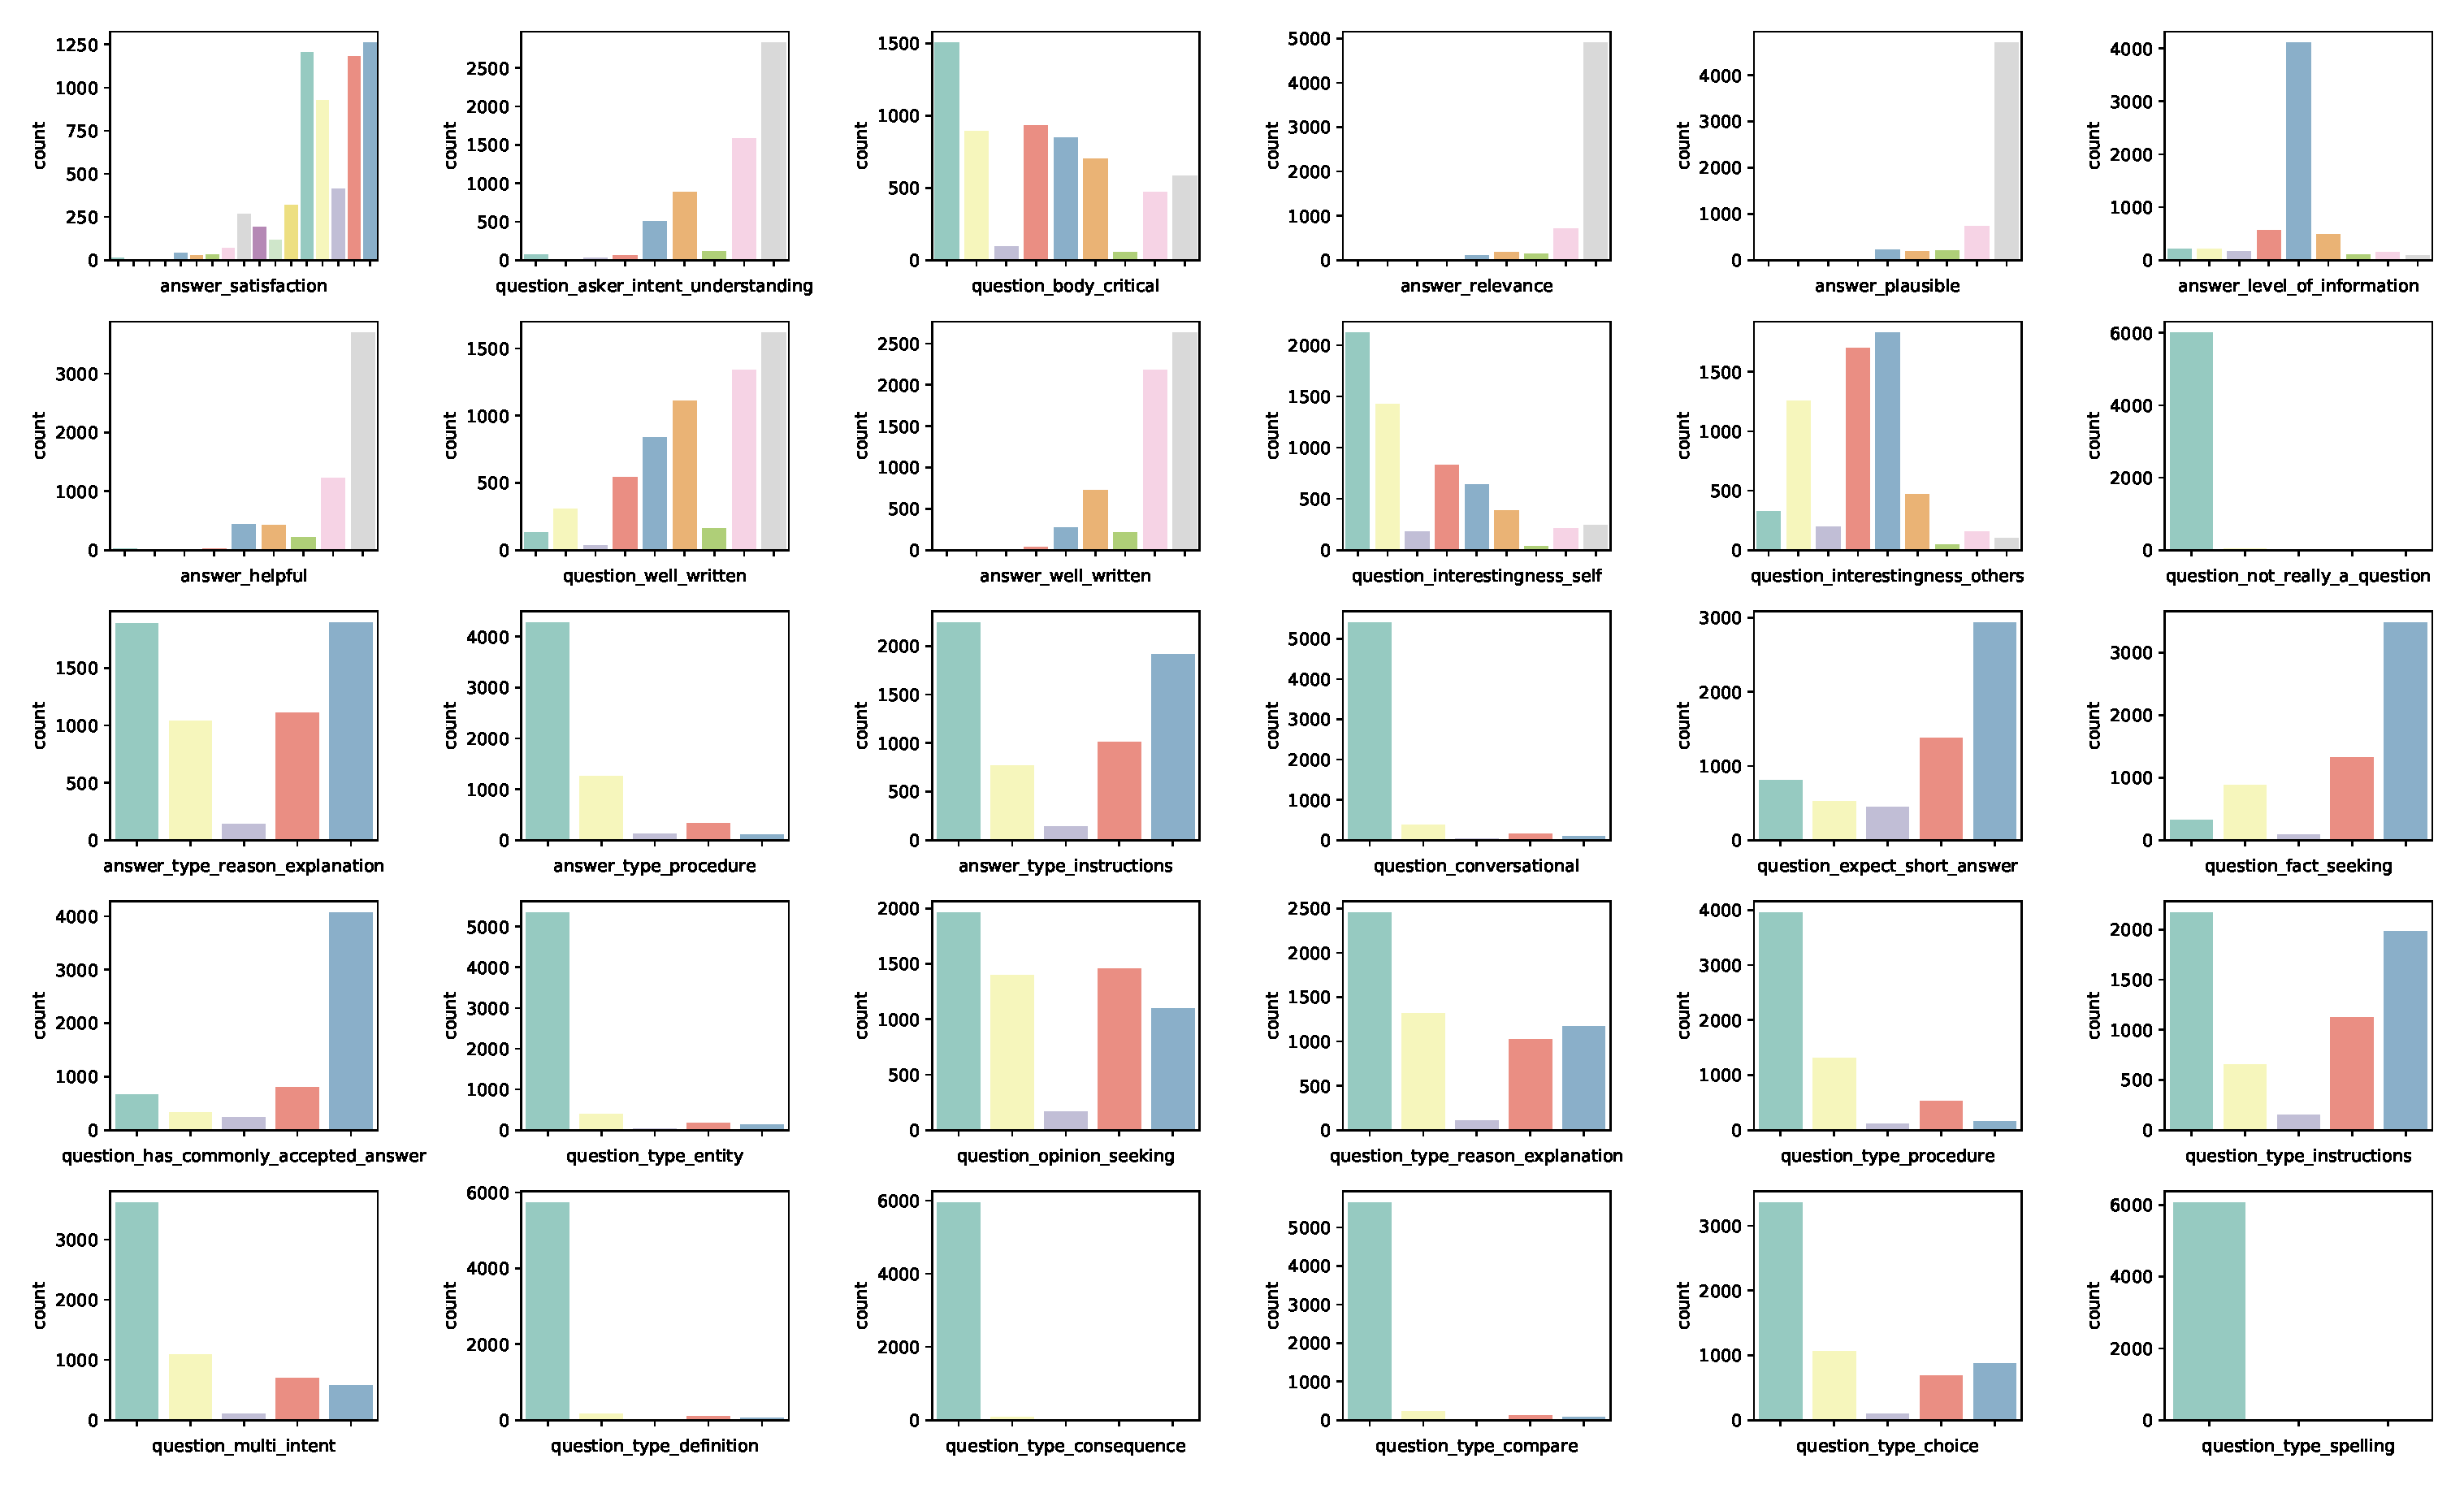
\includegraphics[height=0.75\slideheight]{figures/targets.eps}
    }
\end{slide}
\begin{slide}{Duplicated Questions}
    \begin{itemize}
        \item The competition description has said that:
        \begin{itemize}
            \item \emph{The training data contains rows with some duplicated questions (but with different answers). }
            \item \emph{The test data does not contain any duplicated questions.}
        \end{itemize}
    \end{itemize}
    \begin{table}[htbp]  
        \centering
        \caption{Duplicated Questions}
		\label{tbl:dup_q}
		\begin{tabular}{lc}
			\hline
			Question Title & Count \\
            \hline
            What is the best introductory Bayesian statist...   &12\\
            Important non-technical course for programmers?	    &11\\
            What does mathematics have to do with programm...   &11\\
            How to prevent the "Too awesome to use" syndrome    & 9\\
            How do I deal with a slow and undedicated coll...   & 7\\
            No sound in Ubuntu except at log in	                & 7\\
            What are the benefits of owning a physical book?    & 7\\
            Another instructor is pushing me out of the cl...   & 7\\
            Does "so far, so good" carry a negative connot...   & 6\\
            Good travel games for two players, especially ...   & 6\\
            \dots&-\\
			\hline
		\end{tabular}
	\end{table}
\end{slide}
\begin{slide}{Deal with duplicated questions}
    \begin{itemize}
        \item The question related targets of these records are not always equle.
        \item It's reasonable to set all question related targets of duplicated questions to its mode.
        \begin{itemize}
            \item \emph{t1:\ question_asker_intent_understanding}
            \item \emph{t2:\ question_body_critical}
            \item \emph{t3:\ question_conversational}
        \end{itemize}
    \end{itemize}
    \twocolumn[lineheight=0.5\slideheight, frsep=0cm]{
        \begin{table}
            \centering
            \caption{Example of data before processing}
            \label{tbl:dp_before}
            \begin{tabular}{ccccc}
                \hline
                qa_id	&t1 &t2 &t3 &\dots\\
                \hline
                366	    &1.000000	&1.000000	&0.000000&\dots\\
                2536	&1.000000	&1.000000	&0.666667&\dots\\
                2591	&1.000000	&1.000000	&1.000000&\dots\\
                3349	&1.000000	&1.000000	&1.000000&\dots\\
                5543	&1.000000	&1.000000	&0.000000&\dots\\
                5989	&1.000000	&1.000000	&1.000000&\dots\\
                6041	&0.777778	&1.000000	&0.666667&\dots\\
                6215	&1.000000	&0.888889	&0.333333&\dots\\
                7003	&0.777778	&1.000000	&1.000000&\dots\\
                8328	&1.000000	&1.000000	&0.666667&\dots\\
                8867	&1.000000	&1.000000	&0.666667&\dots\\
                9137	&1.000000	&1.000000	&0.000000&\dots\\
                \hline
            \end{tabular}
        \end{table}
    }{
        \begin{table}
            \centering
            \caption{Example of processed data}
            \label{tbl:dp_after}
            \begin{tabular}{ccccc}
                \hline
                qa_id	&t1 &t2 &t3 &\dots\\
                \hline
                366	    &1.000000	&1.000000	&0.666667&\dots\\
                2536	&1.000000	&1.000000	&0.666667&\dots\\
                2591	&1.000000	&1.000000	&0.666667&\dots\\
                3349	&1.000000	&1.000000	&0.666667&\dots\\
                5543	&1.000000	&1.000000	&0.666667&\dots\\
                5989	&1.000000	&1.000000	&0.666667&\dots\\
                6041	&1.000000	&1.000000	&0.666667&\dots\\
                6215	&1.000000	&1.000000	&0.666667&\dots\\
                7003	&1.000000	&1.000000	&0.666667&\dots\\
                8328	&1.000000	&1.000000	&0.666667&\dots\\
                8867	&1.000000	&1.000000	&0.666667&\dots\\
                9137	&1.000000	&1.000000	&0.666667&\dots\\
                \hline
            \end{tabular}
        \end{table}
    }
\end{slide}
\begin{slide}{Text Data Processing(USE)}
    \begin{itemize}
        \item Since I still don't know too much about nlp, I use \textbf{Google USE}(Universal Sentence Encoder) to convert text data into word vectors here.
        \item It uses a technology called \textbf{''word embedding''} to convert sentences or paragraphs of any length to 512 dimensional float vectors.
    \end{itemize}
    \begin{table}
        \centering
        \caption{Example of Word Vectorization}
        \label{tbl:tx_vec}
        \begin{tabular}{lm{7cm}lm{7cm}}
            \hline
            Name & Before Embedding & After Embedding\\
            \hline
            question_title & What am I losing when using extension tubes instead of a macro lens?&[0.06080658,  0.03104775,  0.02927577, ...]\\
            \hline
            question_body & After playing around with macro photography on-the-cheap (read: reversed lens, rev. lens mounted on a straight lens, passive\dots&[0.06649537, -0.03561426,  0.07933022, ...]\\
            \hline
            answer & I just got extension tubes, so here's the skinny.\textbackslash n\textbackslash n\textbackslash n  ...what am I losing when using tubes...?\textbackslash n\textbackslash n\textbackslash n A very considerable amount of light!  Increasing that distance from the end of the lens to the \dots&[0.03694011, -0.0239582 ,  0.06354006, ...]\\
            \hline
        \end{tabular}
    \end{table}
\end{slide}
\section{Experiment and Analysis}
\begin{slide}{Model Building}
    \begin{itemize}
        \item I tried build serval linear regression model for each target, it doesn't work out.
        \item Then I tried Neural Network, It works better than any kinds of linear regression.
        \item Model: \textbf{Neural Network}
        \begin{itemize}
            \item After serval times tuning, I created a NN with following structure and hyperparameters:
            \item Use sigmoid in output layer to ensure all output are in [0,1] range.
            \item Use dropout to regulize the network, reduce overfit.
        \end{itemize}
    \end{itemize}
    \twocolumn[lineheight=0.3\slideheight]{
        \begin{table}
            \centering
            \caption{Structure of the NN}
            \label{tbl:NN1}
            \begin{tabular}{ccc}
                \hline
                Layer & Output Shape & Activity Function \\
                \hline
                Input & 1536 & -      \\
                Dropout & 1536 & -    \\
                Dense & 512 & elu     \\
                Dropout & 512 & -     \\
                Dense & 30 & elu      \\
                Output & 30 & sigmoid \\ 
                \hline
            \end{tabular}
        \end{table}
    }
    {
        \vspace{0.05\slideheight}
        \begin{table}
            \centering
            \caption{Hyper Params of the NN}
            \label{tbl:NN2}
            \begin{tabular}{cc}
                \hline
                Hyper Param & Value   \\
                \hline
                Loss Function & cross entropy\\
                Optimizer & Adam \\
                Learning Rate & 3e-4 \\
                Dropout Rate & 0.5 \\
                \hline
             \end{tabular}
        \end{table}
    }
\end{slide}
\begin{slide}{Experiment}
    \begin{itemize}
        \item 5 fold cross-validation
        \item Early stopping
        \item \textbf{Evaluate:} Spearman's $\rho$
        \item My Leaderboard Score: 0.346
        \begin{itemize}
            \item \emph{Top Leaderboard Score: 0.465}
        \end{itemize}
    \end{itemize}
    \twocolumn[lineheight=0.4\slideheight]{
        \centering{
        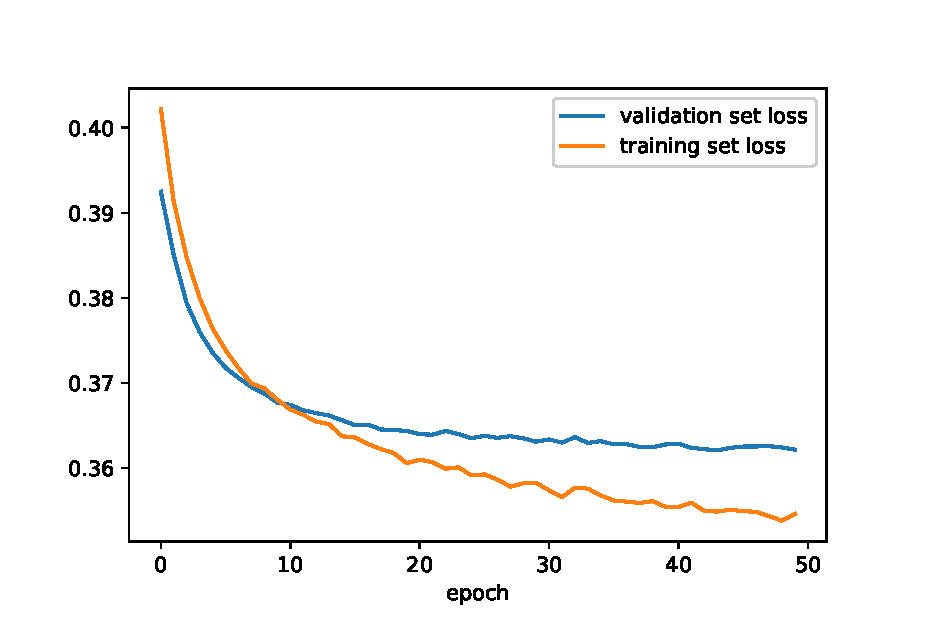
\includegraphics[height=0.4\slideheight]{figures/loss.eps}
        }
    }{
        \centering{
        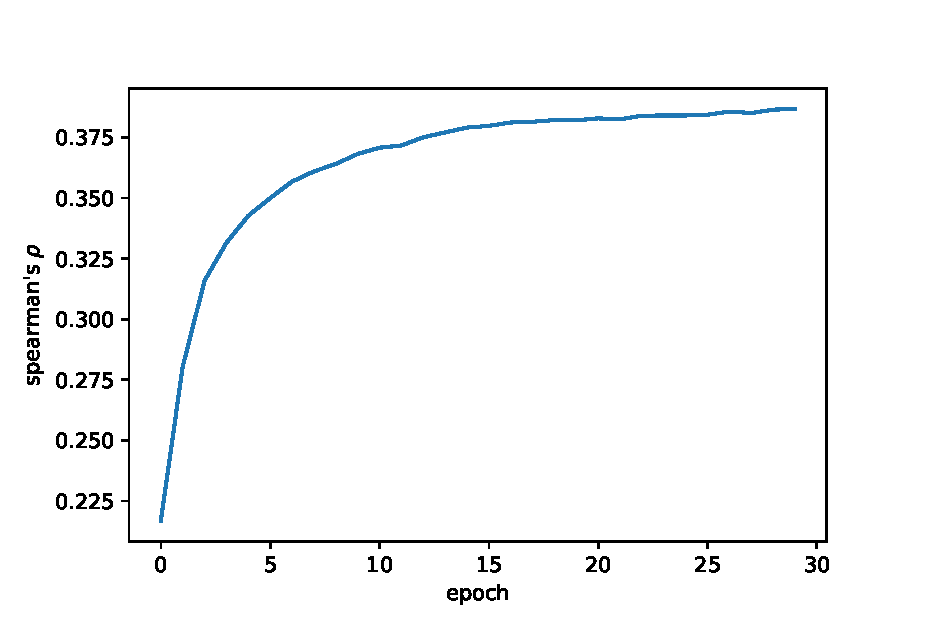
\includegraphics[height=0.4\slideheight]{figures/spearman.eps}
        }
    }
\end{slide}

\section{Conclusion}
\begin{slide}{Conclusion}
    \begin{itemize}
        \item Neural Newwork can work better than linear regression in multi-task learning problem.
        \item It's important to process text data.
        \begin{itemize}
            \item Bag of Word
            \item Word Vector
            \item \dots
        \end{itemize}
        \item Transition Learning may help.
    \end{itemize}
\end{slide}
\begin{emptyslide}{}
	\centering
	\vspace{\stretch{1}}
	{\huge Thank you!}
	\vspace{\stretch{1}}
\end{emptyslide}
\end{document}